\section{Координатный спуск}

\begin{wrapfigure}{r}{0.25\textwidth}
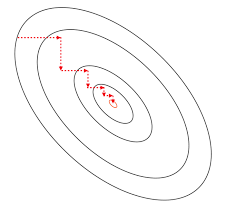
\includegraphics[width=0.9\linewidth]{coordinate_descent.png} 
\caption{Наглядное представление метода}
\label{fig:wrapfig}
\end{wrapfigure}

Рассмотрим один из наиболее простых методов многометрной оптимизации - \textbf{координатный спуск}. На каждой итерации происходит оптимизация по одной переменной, то есть происходит поиск минимума вдоль заданного направления.
Существуют различные порядки перебирания направлений поиска, в простейшем варианте они перебираются по порядку.\\

\begin{remark*}
Алгоритм не требует вычисления производной функции в точке.\\
\end{remark*}

\begin{algo*}
Пусть целевая функция имеет вид:
$f(x): \mathbb{X} \rightarrow \mathbb{R}$, где $\mathbb{X} \subset \mathbb{R}^n$

Задача оптимизации задана в следующем виде:
найти $x_{opt}:f(x_{opt}) = \min\limits_{x\in \mathbb{X}}f(x) = \mu$
\end{algo*}

\begin{itemize}
    \item Задать начальное приближение и точность расчёта: $X_0, \varepsilon$
    \item Рассчитать ${\displaystyle x_{i}^{k+1}={\underset {y\in \mathbb{X}_i }{\operatorname {arg\,min} }}\;f(x_{1}^{k+1},\dots ,x_{i-1}^{k+1},y,x_{i+1}^{k},\dots ,x_{n}^{k})}$
    \item Проверить условие остановки (на усмотрение):
    \begin{itemize}
        \item $|x^{j}-x^{j+1}|<\varepsilon$
        \item $|F(x^{j})-F(x^{j+1})|<\varepsilon$
        \item иначе перейти к пункту 2
    \end{itemize}
\end{itemize}

Таким образом, на каждой итерации будет выполнено
${\displaystyle F({x} ^{0})\geqslant F({x} ^{1})\geqslant F({x} ^{2})\geqslant \dots .}$\\

\textbf{Реализация}
\begin{lstlisting}[language=Python]
def FastSearch(func_index, D, p, e_d, e_f, method):  # F(function), D(set), p(start point), e(error)
    while True:
        p_0 = p
        for index in range(len(p)):
            p = method(func_index, index, D[index][0], D[index][1], p, e_d, e_f)
        if (norm(p_0, p) < e_d) & (Functions[func_index * 2](p_0) - Functions[func_index * 2](p) < e_f):
            break

    best_point = p
    best_value = Functions[func_index * 2](p)
    return best_point, best_value
\end{lstlisting}


\begin{remark*}
Чтобы найти ${\displaystyle x_{i}^{k+1}={\underset {y\in \mathbb {X}_i }{\operatorname {arg\,min} }}\;f(x_{1}^{k+1},\dots ,x_{i-1}^{k+1},y,x_{i+1}^{k},\dots ,x_{n}^{k})}$ будем использовать метод золотого сечения и алгоритм глобальной одномерной оптимизации.   
\end{remark*}

